%%%%%%%%%%%%%%%%%%%%%%%%%%%%%%%%%%%%%%%%%
% University Assignment Title Page 
% LaTeX Template
% Version 1.0 (27/12/12)
%
% This template has been downloaded from:
% http://www.LaTeXTemplates.com
%
% Original author:
% WikiBooks (http://en.wikibooks.org/wiki/LaTeX/Title_Creation)
%
% License:
% CC BY-NC-SA 3.0 (http://creativecommons.org/licenses/by-nc-sa/3.0/)
%
%%%%%%%%%%%%%%%%%%%%%%%%%%%%%%%%%%%%%%%%%
%\title{Title page with logo}
%----------------------------------------------------------------------------------------
%	PACKAGES AND OTHER DOCUMENT CONFIGURATIONS
%----------------------------------------------------------------------------------------

\documentclass[12pt]{article}
\usepackage[english]{babel}
\usepackage[utf8]{inputenc}
\usepackage{natbib}
\usepackage{amsmath}
\usepackage{color}
\usepackage[explicit]{titlesec}
\usepackage[hyphens,spaces,obeyspaces]{url}
\usepackage{graphicx}
\usepackage{caption}
\usepackage{subcaption}
\usepackage{grffile}

\begin{document}

\begin{titlepage}

\newcommand{\HRule}{\rule{\linewidth}{0.5mm}} % Defines a new command for the horizontal lines, change thickness here

\center % Center everything on the page
 
%----------------------------------------------------------------------------------------
%	HEADING SECTIONS
%----------------------------------------------------------------------------------------

\textsc{\LARGE University of St Andrews}\\[1.5cm] % Name of your university/college
\textsc{\Large Distributed Systems}\\[0.5cm] % Major heading such as course name
\textsc{\large CS4103}\\[0.5cm] % Minor heading such as course title

%----------------------------------------------------------------------------------------
%	TITLE SECTION
%----------------------------------------------------------------------------------------

\HRule \\[0.4cm]
{ \huge \bfseries Ring-Based Distributed System}\\[0.4cm] % Title of your document
\HRule \\[1.5cm]
 
%----------------------------------------------------------------------------------------
%	AUTHOR SECTION
%----------------------------------------------------------------------------------------


\Large \emph{Author:}\\
 \textsc{150008022}\\[1cm] % Your name
 
%----------------------------------------------------------------------------------------
%	DATE SECTION
%----------------------------------------------------------------------------------------

{\large \today}\\[2cm] % Date, change the \today to a set date if you want to be precise

%----------------------------------------------------------------------------------------
%	LOGO SECTION
%---------------------------------------------------------------------------------------


\includegraphics[width = 4cm]{images/standrewslogo.png}
 
%----------------------------------------------------------------------------------------

\vfill % Fill the rest of the page with whitespace

\end{titlepage}

\section*{Goal}

To demonstrate an understanding of leader election and mutual exclusion in distributed systems by developing a ring-based distributed social media application.

\tableofcontents
\newpage

\pagenumbering{arabic}
\setcounter{page}{1} 

\section{Initial Set-up}

Java 8 was chosen for this project due to it's friendly socket API, and Maven \cite{maven} was used as the build tool. TDD was implemented with JUnit4 as the the test suite framework.

The project was started with the intention of implementing the bully algorithm as an extension, as it provided fault tolerance with low overhead, but also to provide the option to use the ring based algorithm for comparison.

\subsection{Configuration}

Since each node would be running on an isolated machine, the planned testing environment would involve using \emph{ssh} to start the nodes remotely. Providing the configuration as command line arguments was considered simpler than other methods, and was implemented using the Apache Commons CLI library \cite{apachecli}.

\subsection{Sockets}

Due to different patterns of communication during recovery and regular message passing phases both TCP and UDP were used for this project, as shown in Figure \ref{fig:pattern}.

\noindent TCP was used for communication \textbf{around} the ring:
\begin{enumerate}
    \item Reliable communication avoids token being lost.
    \item Connection is reused frequently between predecessors and successors, justifying handshake overhead.
\end{enumerate}

\noindent UDP was used for communication \textbf{across} the ring: 
\begin{enumerate}
    \item Low communication overhead allows for messages to be sent to multiple nodes quickly, improving recovery time from node failure.
    \item No session maintenance allows coordinator to handle more members in the ring.
\end{enumerate}

\begin{figure}[!h]
\centering
\begin{subfigure}{.5\textwidth}
  \centering
  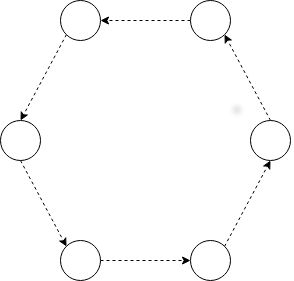
\includegraphics[width=.6\linewidth]{images/tcp}
  \caption{TCP Around Ring}
  \label{fig:tcp}
\end{subfigure}%
\begin{subfigure}{.5\textwidth}
  \centering
  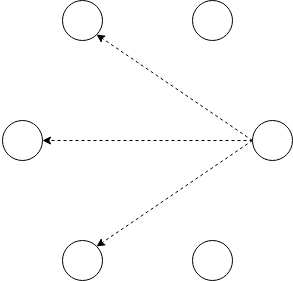
\includegraphics[width=.6\linewidth]{images/udp}
  \caption{UDP Across Ring}
  \label{fig:udp}
\end{subfigure}
\caption{The different types of communication used}
\label{fig:pattern}
\end{figure}

\section{Ring Formation}

\subsection{Initialization}

On initialization, each node sends out join messages to the coordinator. The
joining protocol is similiar to that described in \cite{join}, and is shown in Figure \ref{fig:join}.
Figure \ref{fig:bigjoin} shows how the state of each connection changes over the course of
the joining procedure.

\noindent When node J wants to join the ring:
\begin{enumerate}
    \item J sends join request to coordinator C.
    \item C sends successor to J, telling it to connect to B.
    \item C sends successor to A, telling it to connect to J. 
    \item A disconnects from B, B begins listening for new predecessor.
    \item J connects to B, A connects to J.
\end{enumerate}

\begin{figure}[!ht]
\centering
  \centering
  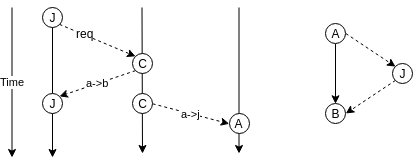
\includegraphics[width=.6\linewidth]{images/join}
  \caption{Joining protocol over time, with topology shown on right.}
\label{fig:join}
\end{figure}


\begin{figure}[!ht]
  \centering
  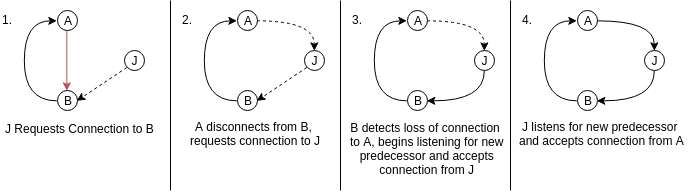
\includegraphics[width=\linewidth]{images/bigflow}
  \caption{State of each connection as a new node joins the ring. The red arrow
shows the edge that is replaced with the new node, and solid and dashed
arrows represent ongoing and pending connections respectively. Either A or
B can be the coordinator in this scenario.}
\label{fig:bigjoin}
\end{figure}

In order for this process to work for a ring network with a single node,
it required another thread to wait on the connection, and the main thread
would then request the connection to itself. For two nodes and more the
joining node would be able to first connect to its new successor once its
predecessor had disconnected from its old successor as shown in figure \ref{fig:bigjoin}.

The coordinator maintains a virtual representation of the network ring
in terms of IDs, and keeps track of the last added node. When a new node
joins, the connection occurs between itself and the last node that was added.
A different heuristic could be used to determine whereabouts the new node
should be inserted into the ring such as %TODO EXPLORE HEURISTICS

\subsection{General Node Recovery}

Node failure is detected whenever either the predecessor or successor of the
failing node attempts to write or read to the relevant TCP socket. The
predecessor is likely first to discover the failure, as they read from the socket
until the token is available. The successor will notice either when it tries to
forward the token or when it tries to send a keepalive.

The successor of the failing node will simply begin listening for a new
predecessor. The predecessor of the failing node will request a new successor
from the coordinator node. The coordinator will then reply with the ID of the node after the failed node for the predeccessor to connect to, at which point normal network behaviour can resume. Figure \ref{fig:failure} shows the topology change when a node fails.

\begin{figure}[!ht]
	\centering
	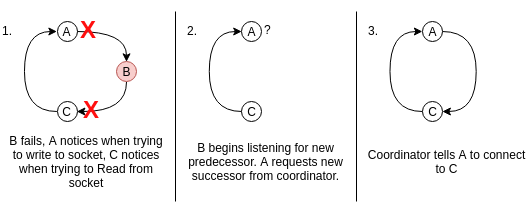
\includegraphics[width=\linewidth]{images/failure}
	\caption{Network topology during the recovery from node B failing. Either A or C are the coordinator in this scenario.}
	\label{fig:failure}
\end{figure}

Since TCP sockets do not provide a method for confirming that a token has been received by next node in the ring at the application level, an acknowledgement mechanism was included in token passing.

\section{Leader/Coordinator Election}

% LIMITATION: Cant have multiple nodes start up at the same time since node assumes itself coordinator

\section{Receive/Send Posts}

\bibliographystyle{unsrt}
\bibliography{mybib}

\end{document}
